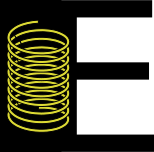
\includegraphics[height=1.5cm]{images/pictograms/elasticity}

\includegraphics[height=1.5cm]{images/pictograms/benchmark}

\lstinputlisting[language=bash,basicstyle=\small]{python_codes/fieldstone_105/keywords.ascii}

\begin{center}
Code at \url{https://github.com/cedrict/fieldstone/tree/master/python_codes/fieldstone_105}
\end{center}

\par\noindent\rule{\textwidth}{0.4pt}

{\sl This stone was developed in collaboration with Zolt{\'a}n Erd{\H{o}}s}. 
\index{contributors}{Z. Erd{\H{o}}s}

\par\noindent\rule{\textwidth}{0.4pt}

%%%%%%%%%%%%%%%%%%%%%%%%%%%%%%%%%%%%%%%%%%%%%%%%%%%%%%%%%%%%%%%%%%%%%%%%%%%%%%%%%%%%%%%%%%%%%%%%%%%%

Under many simplifying approximations (See Section~3.9 of Turcotte \& Schubert book \cite{tusc}), 
the simplest time-independent flexure equation is
\[
D \frac{d^4w(x)}{dx^4} + P \frac{d^2w(x)}{dx^2} + (\rho_m-\rho_c)g w(x) = q(x)
\]
where $w(x)$ is the plate deflection (\si{m}), 
\[
D=\frac{E t^3}{12(1-\nu^2)}
\]
is the flexural rigidity, with $t$ the thickness of the plate (\si{m}), 
$E$ is Young's modulus, $\nu$ is the Poisson ratio, 
$P$ is a horizontal force per unit length (\si{\kg\per\square\metre\square\sec}),  
$q$ is the load (\si{\pascal}), 
$\rho_m$ is the mantle density and $\rho_c$ is the density of the crust (\si{\kg\per\cubic\metre}).
This is a 4th-order ODE. In order to solve it, we will need 4 boundary conditions.

Redo Fig. 3.24 of T\&S. 

We wish to solve this equation on the domain $[0,L_x]$ with the Finite Difference method. 
Indeed the presence of a 4th-order derivative poses quite a few problems for the Finite Element 
method and in this case the FDM is more straighforward to implement (see also 
discussion in Section~2.3 of Buiter \cite{buiter_thesis}). 
The domain is discretised with $n_p$ nodes equally spaced by $h=L_x/(n_p-1)$.

We will need the 2nd- and 4th-order 
derivatives\footnote{\url{https://en.wikipedia.org/wiki/Finite_difference_coefficient}}:
\begin{eqnarray}
\frac{d^2w}{dx^2} &=& \frac{w_{n-1}-2w_n+w_{n+1}}{h^2} 
+{\cal O}(h^3) \\
\frac{d^4w}{dx^4} &=& \frac{w_{n-2}-4w_{n-1}+6w_n-4w_{n+1}+w_{n+2}}{h^4}
+{\cal O}(h^5)
\end{eqnarray}
Both are second-order accurate. We then obtain 
\[
D\frac{w_{n-2}-4w_{n-1}+6w_n-4w_{n+1}+w_{n+2}}{h^4}
+P\frac{w_{n-1}-2w_n+w_{n+1}}{h^2} 
+(\rho_m-\rho_c)g w_n = q_n
\]
or, 
\[
\boxed{
\frac{D}{h^4} w_{n-2}
+\left(-\frac{4D}{h^4}+\frac{P}{h^2}\right)w_{n-1}
+\left(\frac{6D}{h^4}-\frac{2P}{h^2} +(\rho_m-\rho_c)g \right)w_n
+\left(-\frac{4D}{h^4}+\frac{P}{h^2}\right)w_{n+1}
+\frac{D}{h^4} w_{n+2} = q_n
}
\]
One could also multiply this equation by $h^4$ and obtain:
\[
D w_{n-2}
+\left(-4D+Ph^2\right)w_{n-1}
+\left(6D-2Ph^2 +(\rho_m-\rho_c)g h^4 \right)w_n
+\left(-4D+Ph^2\right)w_{n+1}
+D w_{n+2} = q_n h^4
\]
We will formulate this equation for every node $i\in[2,n_p-3]$
in a systematic manner and we will therefore obtain a linear system of equations of the form 
\[
{\bm A} \cdot \vec{w} = \vec{b}
\]
where ${\bm A}$ is an $n_p\times n_p$ matrix (sparse since pentadiagonal) 
and $\vec{b}$ the right-hand side vector. 
The vector $\vec{w}$ contains the $n_p$ deflection unknowns at the nodes of the mesh.

\begin{center}
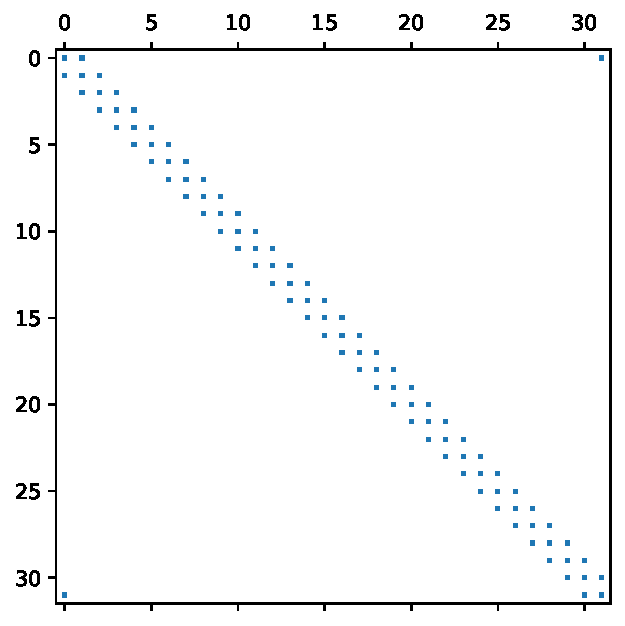
\includegraphics[width=4cm]{python_codes/fieldstone_105/images/matrix}
\end{center}

The four missing lines are addressed when we consider the boundary conditions:
We assume the plate to be very long, and that the load(s) will be 
mostly concentrated around $L_x/2$ . We therefore 
prescribe $w=0$ and $dw/dx=0$ at $x=0$ and $x=L_x$ (i.e. the deflection and 
the slope at the edges of the beam both tend to zero).

The first condition is trivial to impose: set 1 on the diagonal of the 
matrix for $i=0$ and $i=n_p-1$ and the corresponding entries of the rhs to zero. 
The second will have us use the backward derivative on the left for node $i=1$ and 
the forward derivative on the right for node $n_p-2$:
\begin{eqnarray}
\frac{dw}{dx} (x=0)   &\simeq& \frac{-w_0+w_1}{h} \nonumber\\
\frac{dw}{dx} (x=L_x) &\simeq& \frac{-w_{n_p-2}+w_{n_p-1}}{h}
\end{eqnarray}
The two equations will replace the second and before last 
lines in the matrix.

The flexure equation which allows for $D$ to be a function of space is 
\[
\frac{d^2}{dx^2} \left( D(x) \frac{d^2w(x)}{dx^2} \right) + P \frac{d^2w(x)}{dx^2} 
+ (\rho_m-\rho_c)g w(x) = q(x)
\]
Instead of using the expression for a 4th-order derivative we then use the expression 
for a 2nd-order derivative twice. 
Let us temporarily coin $\phi=D(x) \frac{d^2w}{dx^2}$.
Then
\begin{eqnarray}
&&\frac{d^2}{dx^2} \left( D(x) \frac{d^2w(x)}{dx^2} \right)\\
&=& \frac{d^2 \phi}{dx^2} \\
&\simeq& \frac{\phi_{n-1}-2\phi_n+\phi_{n+1}}{h^2} \nonumber\\
&\simeq& \frac{1}{h^2}
\left(
D_{n-1} \frac{w_{n-2}-2w_{n-1}+w_{n}}{h^2}
-2 D_n \frac{w_{n-1}-2w_n+w_{n+1}}{h^2}
+ D_{n+1} \frac{w_{n}-2w_{n+1}+w_{n+2}}{h^2}
\right) \nonumber\\
&=&
\frac{D_{n-1}}{h^4} w_{n-2}
-2\frac{D_{n-1}+D_n}{h^4} w_{n-1}
+\frac{D_{n-1}+4D_n+D_{n+1}  }{h^4} w_n
-2\frac{D_{n}+D_{n+1}}{h^4} w_{n+1}
+\frac{D_{n+1}}{h^4} w_{n+2} \nonumber
\end{eqnarray}
Obviously if $D_{n-1}=D_n=D_{n+1}$ we recover the 
expression above derived with a constant flexural 
rigidity $D$.
The full flexural equation with the variable $D(x)$ then reads as
\begin{eqnarray}
\frac{D_{n-1}}{h^4} w_{n-2}
+\left(-2\frac{D_{n-1}+D_{n}}{h^4}+\frac{P}{h^2}\right)w_{n-1}
+\left(\frac{D_{n-1}+4D_{n}+D_{n+1}}{h^4}-\frac{2P}{h^2} +(\rho_m-\rho_c)g \right)w_n \nonumber\\
+\left(-2\frac{D_{n}+D_{n+1}}{h^4}+\frac{P}{h^2}\right)w_{n+1}
+\frac{D_{n+1}}{h^4} w_{n+2} = q_n
\end{eqnarray}

In what follows the material parameters are those of Fig.~2.2 in Buiter \cite{buiter_thesis}:
$t=10\si{\km}$, $\nu=0.25$, $W=10^{11}\si{\pascal}$, $\rho_m=3250\si{\kg\per\cubic\metre}$, 
$\rho_c=2800\si{\kg\per\cubic\metre}$.

\Literature: Section 11 in Simpson's book \cite{simp17}

%-------------------------------------------------
\subsubsection*{Benchmark 1: line load}

Following Buiter (2000) \cite{buiter_thesis} we consider the case of a lineload.
The lineload $F$ is applied in the middle of the domain and the solution 
is therefore symmetric around $x=L_x/2$.
The analytical solution is given by\footnote{I believe the absolute values
were missing in the thesis.} 
\[
w_{analytical} = \frac{F \alpha^3}{8 D} \exp -\frac{|x|}{\alpha}
\left(
\cos \frac{|x|}{\alpha} + \sin \frac{|x|}{\alpha} 
\right)
\]
with the so-called flexural parameter \index{general}{Flexural Parameter} 
\[
\alpha=\left(\frac{4D}{(\rho_m-\rho_c)g}\right)^{1/4}
\]
which measures the wavelength of the flexure.

\begin{center}
\includegraphics[width=5cm]{python_codes/fieldstone_105/images/buiter}
\includegraphics[width=8cm]{python_codes/fieldstone_105/results/bench1/w.pdf}\\
{\captionfont Left: Taken from \cite{buiter_thesis}}
\end{center}


%-------------------------------------------------
\subsubsection*{Benchmark 2: periodic loading}

For this benchmark we only prescribe $w=0$ at both extremities.
For the second and before last lines of the matrix we resort to 
using forward and backward expressions for the 4th-order 
derivative for simplicity.
The load is given by:
\[
q(x)=\rho_c g h_0 \sin 2\pi \frac{x}{\lambda}
\]
The solution is $w(x)=w_0 \sin 2\pi x/\lambda$, with 
\[
w_0=\frac{h_0}{\frac{\rho_m}{\rho_c}-1+\frac{D}{\rho_c g} (2\pi/\lambda)^4}
\]

\begin{center}
\includegraphics[width=8cm]{python_codes/fieldstone_105/results/bench2/w.pdf}\\
{\captionfont Obtained with $\lambda=0.5Lx$}
\end{center}

%-------------------------------------------------
\subsubsection*{Experiment 3: island}

The load is given by $q(x)=-\rho_c g h_0 \left(1+\cos 2\pi \frac{|x-L_x/2|}{\lambda}\right) $
for $|x-L_x/2|<\lambda/2$ 

\begin{center}
\includegraphics[width=8cm]{python_codes/fieldstone_105/results/exp3/load}
\includegraphics[width=8cm]{python_codes/fieldstone_105/results/exp3/w.pdf}\\
{\captionfont Obtained with $\lambda=0.1$. Left: load; Right: deflection.}
\end{center}



